%%%%%%%%%%%%%%%%%%%%%%%%%%%%%%%%%%%%%%%%%
% Lachaise Assignment
% LaTeX Template
% Version 1.0 (26/6/2018)
%
% This template originates from:
% http://www.LaTeXTemplates.com
%
% Authors:
% Marion Lachaise & François Févotte
% Vel (vel@LaTeXTemplates.com)
%
% License:
% CC BY-NC-SA 3.0 (http://creativecommons.org/licenses/by-nc-sa/3.0/)
% 
%%%%%%%%%%%%%%%%%%%%%%%%%%%%%%%%%%%%%%%%%

%----------------------------------------------------------------------------------------
%	PACKAGES AND OTHER DOCUMENT CONFIGURATIONS
%----------------------------------------------------------------------------------------

\documentclass{article}
\usepackage{float}
%%%%%%%%%%%%%%%%%%%%%%%%%%%%%%%%%%%%%%%%%
% Lachaise Assignment
% Structure Specification File
% Version 1.0 (26/6/2018)
%
% This template originates from:
% http://www.LaTeXTemplates.com
%
% Authors:
% Marion Lachaise & François Févotte
% Vel (vel@LaTeXTemplates.com)
%
% License:
% CC BY-NC-SA 3.0 (http://creativecommons.org/licenses/by-nc-sa/3.0/)
% 
%%%%%%%%%%%%%%%%%%%%%%%%%%%%%%%%%%%%%%%%%

%----------------------------------------------------------------------------------------
%	PACKAGES AND OTHER DOCUMENT CONFIGURATIONS
%----------------------------------------------------------------------------------------

\usepackage{amsmath,amsfonts,stmaryrd,amssymb} % Math packages

\usepackage{enumerate} % Custom item numbers for enumerations

\usepackage[ruled]{algorithm2e} % Algorithms

\usepackage[framemethod=tikz]{mdframed} % Allows defining custom boxed/framed environments

\usepackage{listings} % File listings, with syntax highlighting
\lstset{language=C,keywordstyle={\bfseries \color{blue}}}

%----------------------------------------------------------------------------------------
%	DOCUMENT MARGINS
%----------------------------------------------------------------------------------------

\usepackage{geometry} % Required for adjusting page dimensions and margins

\geometry{
	paper=a4paper, % Paper size, change to letterpaper for US letter size
	top=2.5cm, % Top margin
	bottom=3cm, % Bottom margin
	left=2.5cm, % Left margin
	right=2.5cm, % Right margin
	headheight=14pt, % Header height
	footskip=1.5cm, % Space from the bottom margin to the baseline of the footer
	headsep=1.2cm, % Space from the top margin to the baseline of the header
	%showframe, % Uncomment to show how the type block is set on the page
}

%----------------------------------------------------------------------------------------
%	FONTS
%----------------------------------------------------------------------------------------

\usepackage[utf8]{inputenc} % Required for inputting international characters
\usepackage[T1]{fontenc} % Output font encoding for international characters

\usepackage{XCharter} % Use the XCharter fonts

%----------------------------------------------------------------------------------------
%	COMMAND LINE ENVIRONMENT
%----------------------------------------------------------------------------------------

% Usage:
% \begin{commandline}
%	\begin{verbatim}
%		$ ls
%		
%		Applications	Desktop	...
%	\end{verbatim}
% \end{commandline}

\mdfdefinestyle{commandline}{
	leftmargin=10pt,
	rightmargin=10pt,
	innerleftmargin=15pt,
	middlelinecolor=black!50!white,
	middlelinewidth=2pt,
	frametitlerule=false,
	backgroundcolor=black!5!white,
	frametitle={Command Line},
	frametitlefont={\normalfont\sffamily\color{white}\hspace{-1em}},
	frametitlebackgroundcolor=black!50!white,
	nobreak,
}

% Define a custom environment for command-line snapshots
\newenvironment{commandline}{
	\medskip
	\begin{mdframed}[style=commandline]
}{
	\end{mdframed}
	\medskip
}

%----------------------------------------------------------------------------------------
%	FILE CONTENTS ENVIRONMENT
%----------------------------------------------------------------------------------------

% Usage:
% \begin{file}[optional filename, defaults to "File"]
%	File contents, for example, with a listings environment
% \end{file}

\mdfdefinestyle{file}{
	innertopmargin=1.6\baselineskip,
	innerbottommargin=0.8\baselineskip,
	topline=false, bottomline=false,
	leftline=false, rightline=false,
	leftmargin=2cm,
	rightmargin=2cm,
	singleextra={%
		\draw[fill=black!10!white](P)++(0,-1.2em)rectangle(P-|O);
		\node[anchor=north west]
		at(P-|O){\ttfamily\mdfilename};
		%
		\def\l{3em}
		\draw(O-|P)++(-\l,0)--++(\l,\l)--(P)--(P-|O)--(O)--cycle;
		\draw(O-|P)++(-\l,0)--++(0,\l)--++(\l,0);
	},
	nobreak,
}

% Define a custom environment for file contents
\newenvironment{file}[1][File]{ % Set the default filename to "File"
	\medskip
	\newcommand{\mdfilename}{#1}
	\begin{mdframed}[style=file]
}{
	\end{mdframed}
	\medskip
}

%----------------------------------------------------------------------------------------
%	NUMBERED QUESTIONS ENVIRONMENT
%----------------------------------------------------------------------------------------

% Usage:
% \begin{question}[optional title]
%	Question contents
% \end{question}

\mdfdefinestyle{question}{
	innertopmargin=1.2\baselineskip,
	innerbottommargin=0.8\baselineskip,
	roundcorner=5pt,
	nobreak,
	singleextra={%
		\draw(P-|O)node[xshift=1em,anchor=west,fill=white,draw,rounded corners=5pt]{%
		Question \theQuestion\questionTitle};
	},
}

\newcounter{Question} % Stores the current question number that gets iterated with each new question

% Define a custom environment for numbered questions
\newenvironment{question}[1][\unskip]{
	\bigskip
	\stepcounter{Question}
	\newcommand{\questionTitle}{~#1}
	\begin{mdframed}[style=question]
}{
	\end{mdframed}
	\medskip
}

%----------------------------------------------------------------------------------------
%	WARNING TEXT ENVIRONMENT
%----------------------------------------------------------------------------------------

% Usage:
% \begin{warn}[optional title, defaults to "Warning:"]
%	Contents
% \end{warn}

\mdfdefinestyle{warning}{
	topline=false, bottomline=false,
	leftline=false, rightline=false,
	nobreak,
	singleextra={%
		\draw(P-|O)++(-0.5em,0)node(tmp1){};
		\draw(P-|O)++(0.5em,0)node(tmp2){};
		\fill[black,rotate around={45:(P-|O)}](tmp1)rectangle(tmp2);
		\node at(P-|O){\color{white}\scriptsize\bf !};
		\draw[very thick](P-|O)++(0,-1em)--(O);%--(O-|P);
	}
}

% Define a custom environment for warning text
\newenvironment{warn}[1][Warning:]{ % Set the default warning to "Warning:"
	\medskip
	\begin{mdframed}[style=warning]
		\noindent{\textbf{#1}}
}{
	\end{mdframed}
}

%----------------------------------------------------------------------------------------
%	INFORMATION ENVIRONMENT
%----------------------------------------------------------------------------------------

% Usage:
% \begin{info}[optional title, defaults to "Info:"]
% 	contents
% 	\end{info}

\mdfdefinestyle{info}{%
	topline=false, bottomline=false,
	leftline=false, rightline=false,
	nobreak,
	singleextra={%
		\fill[black](P-|O)circle[radius=0.4em];
		\node at(P-|O){\color{white}\scriptsize\bf i};
		\draw[very thick](P-|O)++(0,-0.8em)--(O);%--(O-|P);
	}
}

% Define a custom environment for information
\newenvironment{info}[1][Info:]{ % Set the default title to "Info:"
	\medskip
	\begin{mdframed}[style=info]
		\noindent{\textbf{#1}}
}{
	\end{mdframed}
} % Include the file specifying the document structure and custom commands

%----------------------------------------------------------------------------------------
%	ASSIGNMENT INFORMATION
%----------------------------------------------------------------------------------------

\title{CS426: Project \#4 Report} % Title of the assignment

\author{Doruk Çakmakçı\\ \texttt{21502293}} % Author name and email address

\date{Bilkent University --- \today} % University, school and/or department name(s) and a date

%----------------------------------------------------------------------------------------

\begin{document}

\maketitle % Print the title

%----------------------------------------------------------------------------------------
%	INTRODUCTION
%----------------------------------------------------------------------------------------

\section{Introduction} 
\qquad Sparseness of a matrix is an important concern for matrix multiplication. Because, the zero-valued elements of a matrix does not contribute to the output of matrix multiplication. For improving space complexity of a program, 2D sparse matrices are stored using three arrays instead of a two dimensional array. One of the arrays store an index value( an implementation detail which has no spatial meaning) corresponding to the first non-zero element for each row. The second array has elements which are the indexed by the index value mentioned above which holds the column of the corresponding matrix element. The third array hold the values corresponding to the row and columns of the matrix and indexed in the like manner with the second array. In the following analysis, first array is referred as row\_ptr, the second array is referenced as col\_ind and the third array is referred as values array\\
\null \qquad Our goal in this project is to parallelize sparse matrix vector multiplication using GPU parallelism. NVIDIA CUDA is used as the parallelization tool.

\section{Parallelization Strategy} 
\qquad The algorithm is parallelized by distributing the elements of the row\_ptr array to the threads. To be concise, 1D block distribution(as input data decomposition technique) is used as the parallelization strategy. Each Thread computes the start(inclusive) and end(exclusive) indices for its own computation. In order to ensure load balancing, first the quotient of $number\_of\_rows / number\_of\_threads$ is distributed to all threads. The remainder of this division is distributed to threads with respect to the id's of the threads. Therefore the maximum difference in computation(in terms of rows) is for any two thread. However, since rows can have drastically different number of non-zero elements( some have no elements at all), load balancing can only be done by distributing the values array to the threads. But, using a parallelization strategy that uses values array distribution is very hard to implement and introduces more space requirements. If the this algorithm would be used in a real-time system, then values array distribution would be more feasible in terms of running time requirements.\\
\null \qquad CUDA uses grids of blocks and blocks of threads. For this implementation, grids consist of 1 block and blocks contain 1D thread blocks. Also there are number\_of\_threads thread blocks.This scheme is bounded by the architectural limits. In the CUDA documentation, it is stated that a block can have at most 1024 threads inside it. However, in my analysis, I have seen that 1024 threads is enough for a good parallelism.\\

\section{Notes} 
\qquad In the following analysis, Amdahl's law is used to compute the speedup and efficiency of the parallel algorithm. Instead of using Amdahl's law, one can implement the sequential version of the sparse matrix vector multiplication. However, to measure speedup, one must use the best algorithm(in terms of time complexity). Since the best implementation is a relatively contextual, Amdahl's law is used. The sequential part of the algorithm consists of reading the sparse matrix from file. The parallelizable part of the implementation is the sparse matrix vector multiplication. Since there is no sequential implementation of the algorithm for this project, an approximate analysis for the proportion of the parallelizable part of the  implementation would be dependent to the iteration count. The sequential part of the algorithm contains $ 3 * k$( k is just a proportionality constant 3 is for creating the three arrays mentioned previously). The parallelizable part of the algorithm contains $ 1.5 * (iteration\_count) * k$(1.5 is for copying from and to device memory and the computation on the elements. this factor is multiplied with iteration\_count to scale up).

\section{Figures}
\subsection{cavity02.mtx}
\subsubsection{Parallel Running Time vs # of Iterations}

\begin{figure}[H]
\centering
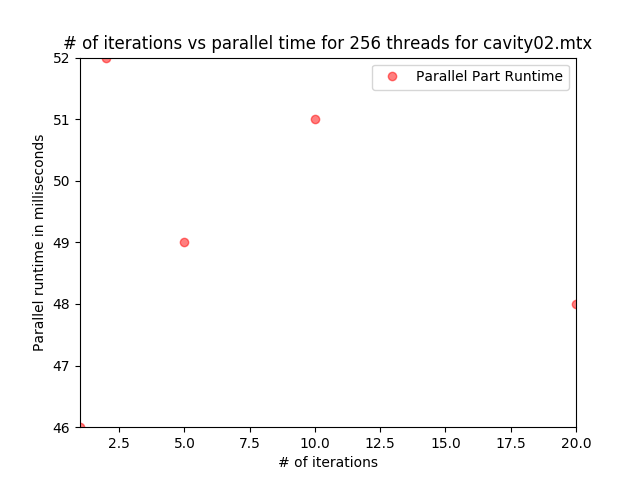
\includegraphics[width=\linewidth]{assets/cavity_iter_parallel.png}
\label{fig:test1}
\vspace{-2pt}
\end{figure}

\null \qquad From the figure we can see that the number of iterations do not monotonically increase the running part of the parallel algorithm. I did not foresee this result since increasing the number of iterations should increase the running time of the program drastically. For this case, it may be the case that the size of the cavity02 matrix is small and does not introduce a lot of overhead while increasing iteration. As a last minute note I have found out that the selected iteration counts for this plot are not representative of the effect of number of iterations on the parallel running time. The following results (tested using the same parameters) are more representative:
\begin{itemize}
    \item \textbf{100 iterations:} parallel part running  time is 60ms
    \item \textbf{1000 iterations:} parallel part running  time is 102ms
    \item \textbf{10000 iterations:} parallel part running  time is 570ms
\end{itemize}
We can see that 1 iteration does not introduce a significant overhead but testing the program using the powers of 10 gives better results.

\subsubsection{Parallel Running Time vs # of Threads}

\begin{figure}[H]
\centering
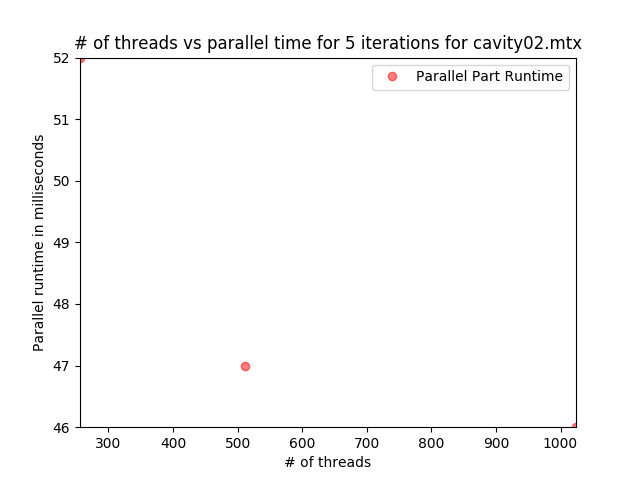
\includegraphics[width=\linewidth]{assets/cavity_thr_parallel.png}
\label{fig:test1}
\vspace{-2pt}
\end{figure}

\null \qquad As expected, we see that the number of threads used is significant in terms of running time(the outcome is dependent to the size of the input and over-decomposing the inputs can also generate an overhead higher than the benefit of the parallelization). As the number of threads is increased, the running time of the program decreases.

\subsubsection{Speedup}

\begin{figure}[H]
\centering
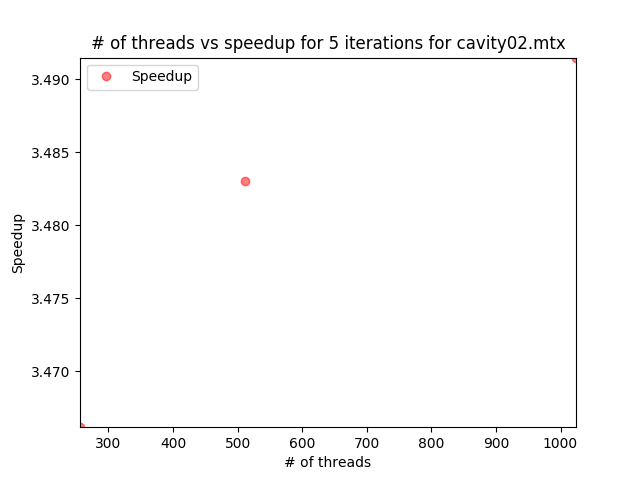
\includegraphics[width=\linewidth]{assets/cavity_thr_speedup.png}
\label{fig:test1}
\vspace{-2pt}
\end{figure}

\null \qquad Keeping in mind that the speedup is bounded by the number of processors and the plotted speedup is theoretical and approximate, the results are not good. However a more pervasive analysis of the implementation(using the best sequential implementation of sparse matrix vector product and calculating the speedup as $sequential\_time / parallel\_time$) may yield a better result. From another perspective, using cuda cores as the number of processors in the Amdahl's law is may not be feasible since some CUDA cores may be using the physical processor.

\subsubsection{Efficiency}

\begin{figure}[H]
\centering
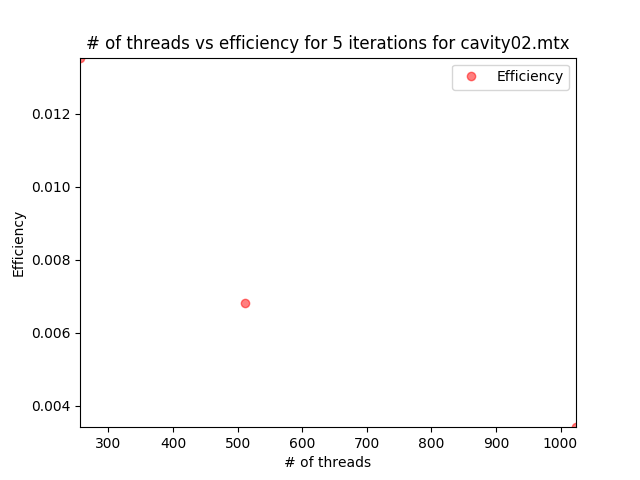
\includegraphics[width=\linewidth]{assets/cavity_thr_eff.png}
\label{fig:test1}
\vspace{-2pt}
\end{figure}

\null \qquad Since efficiency is the speedup per processor, we can say that the speedup per processor drops with respect to the number of threads used.  Speedup tends to saturate with respect to the number of threads(if more threads are used it is speculated that speedup would converge(saturate)) and efficiency drops as a consequence. We can see this phenomena in this plot. Also this system is not cost-optimal since the efficiency is not constant with respect to number of processors and speedup per processor changes.


\subsection{fidapm08.mtx}
\subsubsection{Parallel Running Time vs # of Iterations}

\begin{figure}[H]
\centering
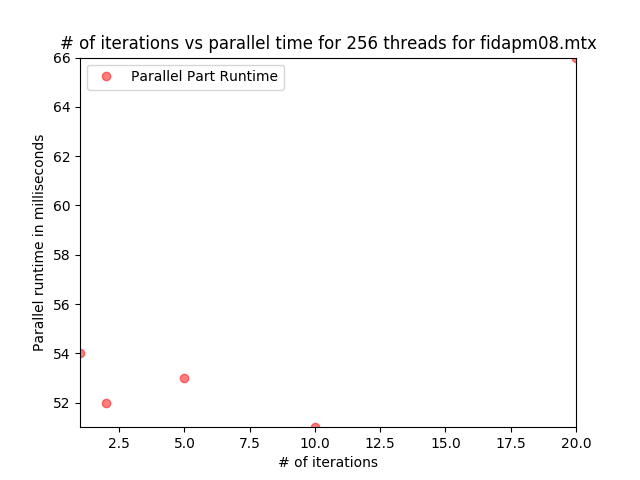
\includegraphics[width=\linewidth]{assets/fidapm08_iter_parallel.png}
\label{fig:test1}
\vspace{-2pt}
\end{figure}

\null \qquad We can see that the parallel running times are increased slightly with respect to the size of the input.

\subsubsection{Parallel Running Time vs # of Threads}

\begin{figure}[H]
\centering
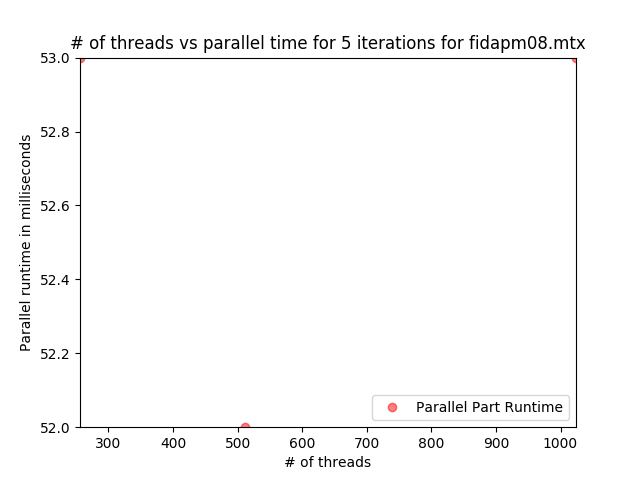
\includegraphics[width=\linewidth]{assets/fidapm08_thr_parallel.png}
\label{fig:test1}
\vspace{-2pt}
\end{figure}

\null \qquad The parallel running time is almost constant with respect to these number of threads but since this only a small part of a big spectrum no influential analysis can be made from this graph.

\subsubsection{Speedup}

\begin{figure}[H]
\centering
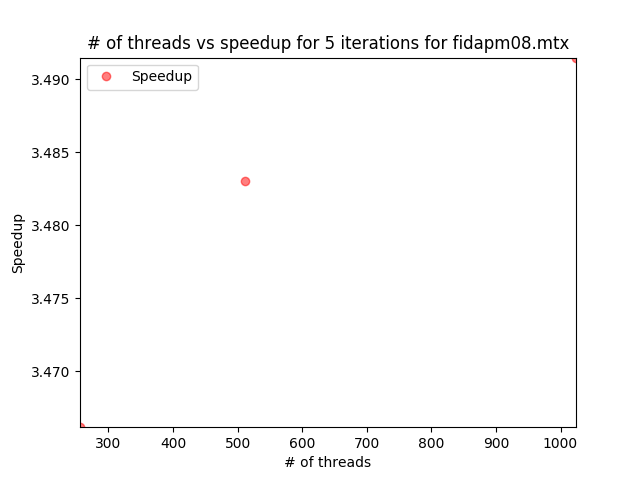
\includegraphics[width=\linewidth]{assets/fidapm08_thr_speedup.png}
\label{fig:test1}
\vspace{-2pt}
\end{figure}

\null \qquad A similar analysis as the cavity02 matrix can be made.

\subsubsection{Efficiency}

\begin{figure}[H]
\centering
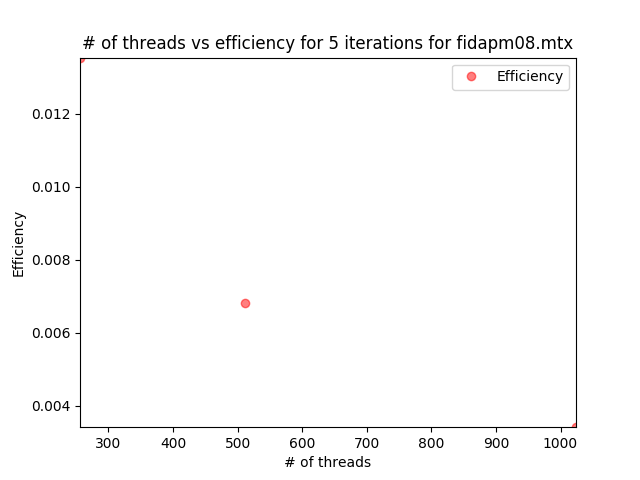
\includegraphics[width=\linewidth]{assets/fidapm08_thr_eff.png}
\label{fig:test1}
\vspace{-2pt}
\end{figure}

\null \qquad A similar analysis as the cavity02 matrix can be made.


\subsection{fidapm11.mtx}
\subsubsection{Parallel Running Time vs # of Iterations}

\begin{figure}[H]
\centering
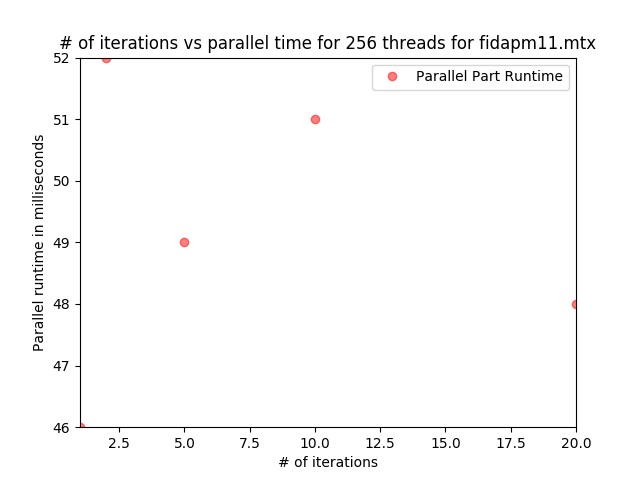
\includegraphics[width=\linewidth]{assets/fidapm11_iter_parallel.png}
\label{fig:test1}
\vspace{-2pt}
\end{figure}

\null \qquad A similar analysis as the cavity02 matrix can be made.

\subsubsection{Parallel Running Time vs # of Threads}

\begin{figure}[H]
\centering
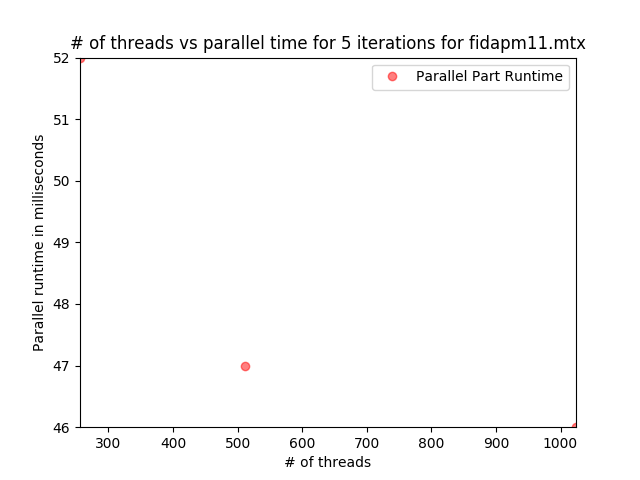
\includegraphics[width=\linewidth]{assets/fidapm11_thr_parallel.png}
\label{fig:test1}
\vspace{-2pt}
\end{figure}

\null \qquad A similar analysis as the cavity02 matrix can be made.

\subsubsection{Speedup}

\begin{figure}[H]
\centering
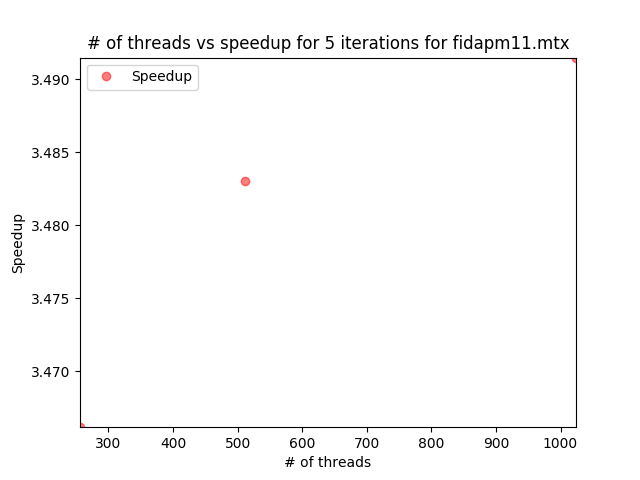
\includegraphics[width=\linewidth]{assets/fidapm11_thr_speedup.png}
\label{fig:test1}
\vspace{-2pt}
\end{figure}

\null \qquad A similar analysis as the cavity02 matrix can be made.

\subsubsection{Efficiency}

\begin{figure}[H]
\centering
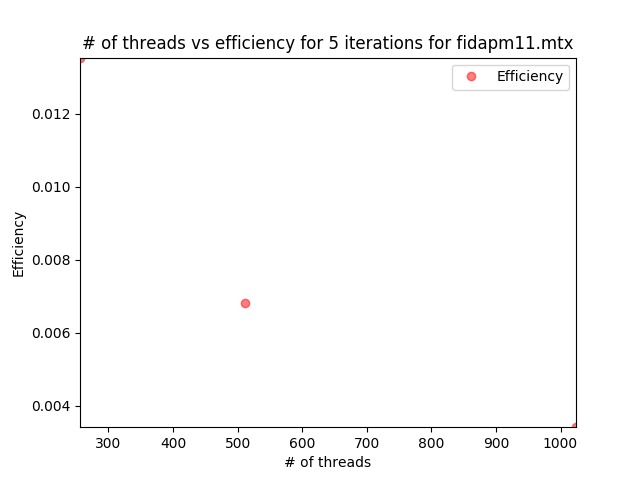
\includegraphics[width=\linewidth]{assets/fidapm11_thr_eff.png}
\label{fig:test1}
\vspace{-2pt}
\end{figure}

\null \qquad A similar analysis as the cavity02 matrix can be made.

\end{document}